\addcontentsline{toc}{chapter}{Gabarito}
\chapter*{Gabarito}

\addcontentsline{toc}{section}{Capítulo 1 - Afinal, o que é um robô?}
\section*{Capítulo 1 - Afinal, o que é um robô?}

    \subsection*{1)}
    Perguntar ao professor.
        \begin{multicols}{3}
            \begin{figure}[H]
            \caption{Praticar esportes}
     
            \centering 
            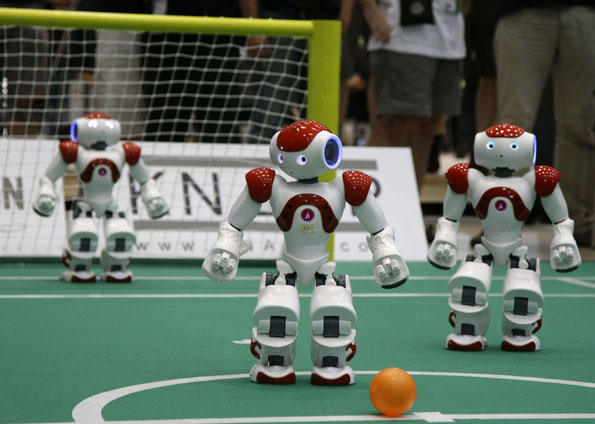
\includegraphics[width=5cm]{Figuras/NAO.jpg}
            \label{figura:NAO.jpeg}
            \end{figure}
        
            \begin{figure}[H]
            \caption{Robô que anda em terra e na água, pode ser utilizado para localizar coisas}
     
            \centering 
            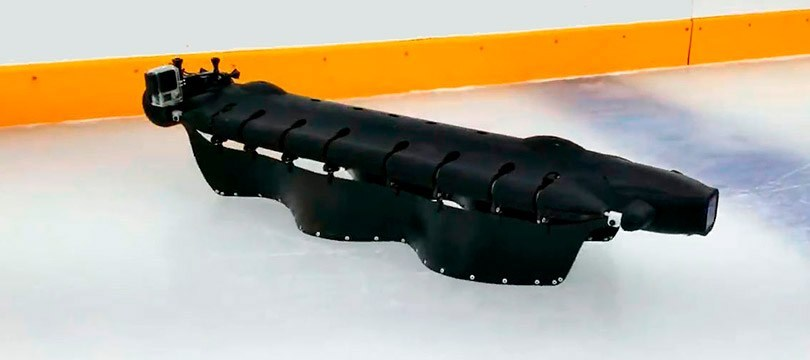
\includegraphics[width=5cm]{Figuras/anfibio.jpg}
            \label{figura:anfibio.jpeg}
            \end{figure}

            \begin{figure}[H]
            \caption{Sophie, estudos sobre inteligência artificial}
     
            \centering 
            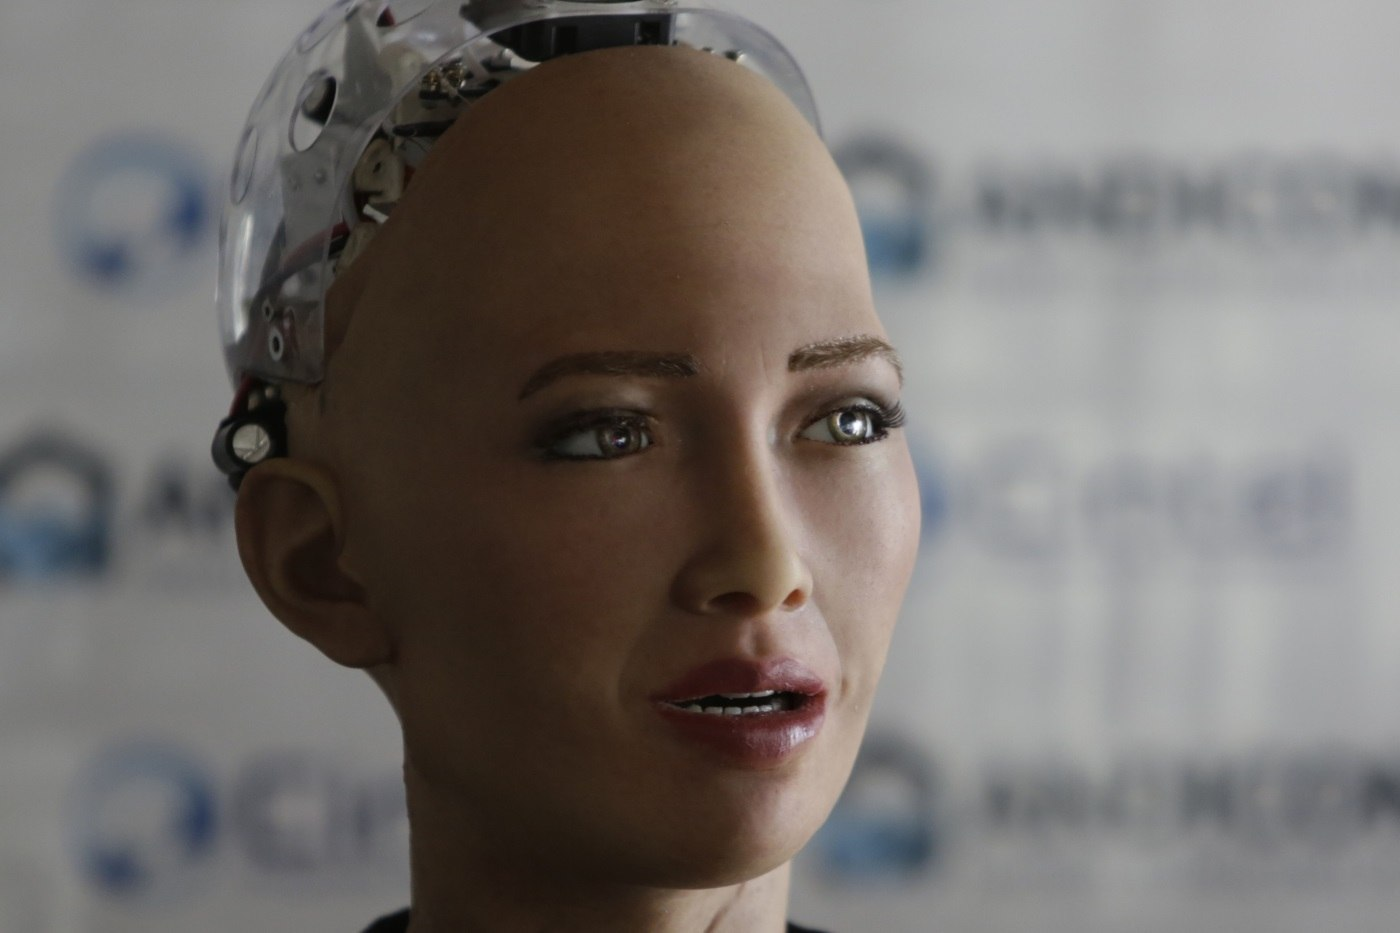
\includegraphics[width=6cm]{Figuras/sophie.jpeg}
            \label{figura:sophie.jpeg}
            \end{figure}
        \end{multicols}
        
     \subsection*{2)}
        Não, termômetros não são capazes de tomar decisões, de agir sobre o meio, ele é somente uma ferramenta para calcular e visualizar a temperatura ambiente.
        
    \subsection*{3)} Perguntar ao professor.
        
    \subsection*{4)}
        A geladeira sabe quando a porta está aberta e quando está fechada, e nisso decide se acende ou apaga a luz de dentro dela, porém isso não passa apenas de algum circuito lógico. Uma boneca que fala ou se mexe sozinha é bem "robótica" por dentro, mas é incapaz de perceber os seus arredores e realizar ações não repetitivas (tenha certeza que o fabricante disse que a boneca deveria se mexer, caso não venha explicitado, pode ser caso de assombração!).
        
    \subsection*{\textbf{Desafio}}
        Perguntar ao professor.
        

\addcontentsline{toc}{section}{Capítulo 2 - Algoritmos e fluxograma}        
\section*{Capítulo 2 - Algoritmos e fluxograma}

    \subsection*{1)} Perguntar ao professor.
    
    \subsection*{2)} Letra a.
    
    \subsection*{3)} Existem varias soluções corretas, aqui vai uma sugestão, busque sempre ser detalhista.
        \begin{figure}[H]
        \centering
        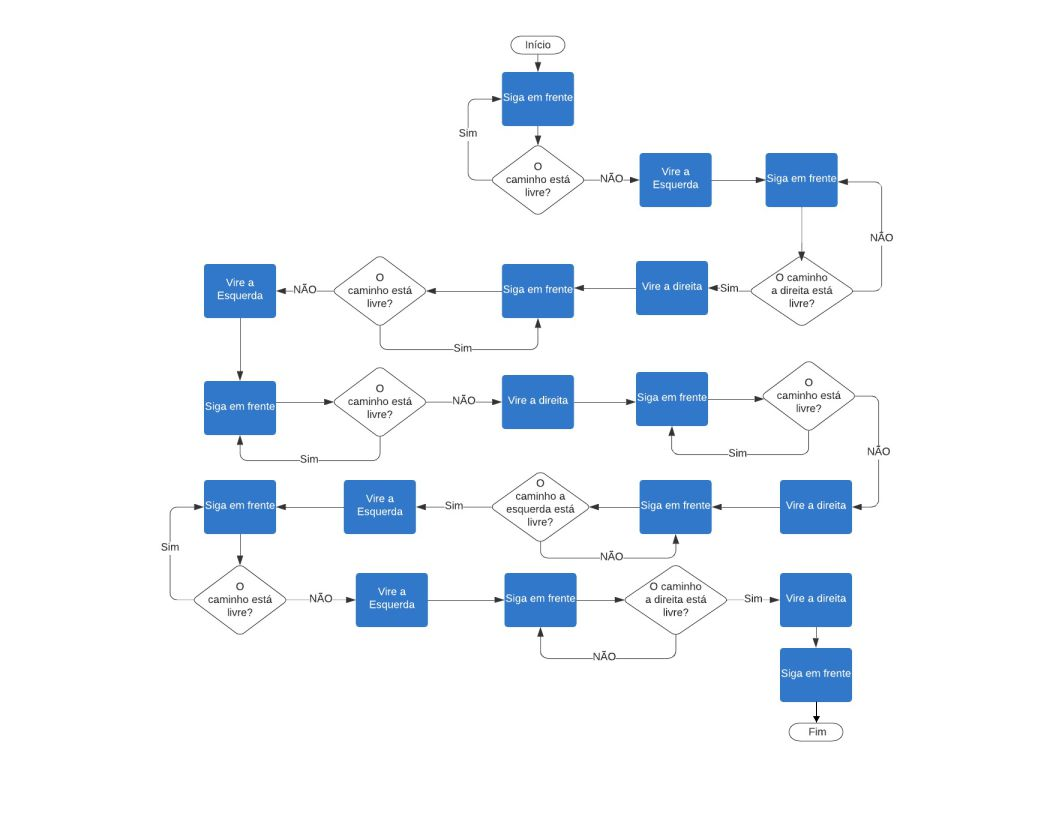
\includegraphics[width=18cm]{Figuras/sollab.jpg}
        \label{figura:solução.jpg}
        \end{figure}
    
\addcontentsline{toc}{section}{Capítulo 3 - Tela LCD}      
\section*{Capítulo 3 - Tela LCD}
    
    \subsection*{1)} Para descobrir o meio da tela, basta dividir as dimensões da tela LCD por dois, logo, o ponto central terá as seguintes coordenadas: \\ x = 128 / 2 = 64 \\ y = 64 / 2 = 32
    

    \lstinputlisting[language=C] {codigos_gabarito/capitulo_3/exercicio-3.1.c}
    
    \subsection*{2)} Letra d.
    
    \subsection*{3)} 
    
    %Ajustar o recuo da esquerda.
     a) 10 pixels.\\
    \indent b) 25 pixels.

    \subsection*{Desafio) Perguntar ao professor.}

\addcontentsline{toc}{section}{Capítulo 4 - Movimentação} 
\section*{Capítulo 4 - Movimentação}

    \subsection*{1)}
    Letra c.
    
    \subsection*{2) (Existe mais de uma solução para este exercício)}

 \lstinputlisting[language=C]{codigos_gabarito/capitulo_4/exercicio-2.c}

    \textsl{Como a distância a ser percorrida pelo robô é equivalente ao lado do quadrado, o valor dentro dos parênteses da função ``sparki.moveForward()'' é 5.}
    
    \subsection*{3) (Existe mais de uma solução para este exercício)} 
    
     \lstinputlisting[language=C]{codigos_gabarito/capitulo_4/exercicio-3.c}
    
    \subsection*{4)}
    Letra d.
    
    \subsection*{5)}
    
 \lstinputlisting[language=C]{codigos_gabarito/capitulo_4/exercicio-5.c}
 
    \subsection*{6)}
    \textsl{Este código abre totalmente as garras e depois as fecha durante 1 segundo. Poderia simular as garras pegando um objeto.}
    
    \subsection*{Desafio) Perguntar ao professor.}
    
\addcontentsline{toc}{section}{Capítulo 5 - Variáveis} 
\section*{Capítulo 5 - Variáveis}

    \subsection*{1)}
 \lstinputlisting[language=C]{codigos_gabarito/capitulo_5/exercicio-1.c}
 
    \subsection*{2)}
 \lstinputlisting[language=C]{codigos_gabarito/capitulo_5/exercicio-2.c}


 %   \subsection*{3)}
 %   \begin{lstlisting}[language=C]

%#include <Sparki.h>;

%int distancia;

%void setup()
%{
%}

%void loop()
%{
%    distancia = sparki.ping();
%    distancia -=10;
%    sparki.moveForward(distancia);
%}
%\end{lstlisting}

%   } não sei se isso deveria estar aq, mas caso fosse para estar então não apaguei
    
    \subsection*{Desafio) Perguntar ao professor.}

 \lstinputlisting[language=C]{codigos_gabarito/capitulo_5/desafio.c}

\addcontentsline{toc}{section}{Capítulo 6 - Ultrassom} 
\section*{Capítulo 6 - Ultrassom}

    \subsection*{1)}
    
        Conhecendo a velocidade do som, que é aproximadamente 340 m/s, nós sabemos quantos metros o som percorre em 1 segundo.
        Se conhecermos também quanto tempo levou para a onda ir e voltar, podemos fazer uma \textbf{regra de três} para descobrir quantos metros a onda andou.
        Ou seja, o som faz: 
        \par
        \textbf{340} metros => \textbf{1} segundo 
        \par
        \textbf{x} metros => \textbf{t} segundo(s) \par
        Sendo \textbf{x} a quantidade de metros que a onda andou e \textbf{t} quantos segundos foram necessários para a onda fazer esse trajeto.
        Então, podemos achar \textbf{x} multiplicando as diagonais da regra de 3 e igualando-as, assim: 
        \par
        \textbf{340} . \textbf{t} = \textbf{x} . \textbf{1} 
        \par
        Agora, isolamos o \textbf{x}:
        \par
        \textbf{x} = 340t
        \par
        Mas devemos levar em consideração que a onda vai até o objeto e volta até o sensor, por isso a distância do sensor até o objeto é metade do \textbf{x} encontrado:
        \par
        \textbf{x} = 340t/2 = 170t
        \par
        E esse é o nosso resultado!
    
    \subsection*{2)}
    
 \lstinputlisting[language=C]{codigos_gabarito/capitulo_6/exercicio-2.c}

    \subsection*{3)}
    
 \lstinputlisting[language=C]{codigos_gabarito/capitulo_6/exercicio-3.c}

    
    \subsection*{4)}
    
 \lstinputlisting[language=C]{codigos_gabarito/capitulo_6/exercicio-4.c}

    
    \subsection*{Desafio) Perguntar ao professor.}

\addcontentsline{toc}{section}{Capítulo 7 - If e Else}
\section*{Capítulo 7 - If e Else}

    \subsection*{1)} x = 2; y = 1; Falso.

    \subsection*{2)} Verdadeiro; Verdadeiro.

    \subsection*{3)} Verdadeiro.

    \subsection*{4)} Letra b.
    
    \subsection*{5) (Existe mais de uma solução para este exercício)}
    
 \lstinputlisting[language=C]{codigos_gabarito/capitulo_7/exercicio-5.c}
    
    \subsection*{6)}
    
 \lstinputlisting[language=C]{codigos_gabarito/capitulo_7/exercicio-6.c}


    \subsection*{Desafio) Em caso de dúvidas, perguntar ao professor.}

\addcontentsline{toc}{section}{Capítulo 8 - Infravermelho}
\section*{Capítulo 8 - Infravermelho}

    \subsection*{1)}
    A resposta a seguir é apenas um exemplo, pode-se utilizar de quaisquer botões disponíveis para controlar o robô.
    
 \lstinputlisting[language=C]{codigos_gabarito/capitulo_8/exercicio-1.c}

    
    \subsection*{2)}
    
 \lstinputlisting[language=C]{codigos_gabarito/capitulo_8/exercicio-2.c}
 
    O passo 1 do programa é quando recebemos o primeiro número da conta, no segundo passo devemos definir se a operação é de adição ou de subtração, no terceiro passo escolhemos o segundo número e por último fazemos os cálculos e mostramos o resultado na tela LCD. Caso o usuário não aperte os botões corretos, o programa detecta a falha e repete o último passo.
    
    \subsection*{3)}
 
 \lstinputlisting[language=C]{codigos_gabarito/capitulo_8/exercicio-3.c}

    
    \subsection*{4)}
    
 \lstinputlisting[language=C]{codigos_gabarito/capitulo_8/exercicio-4.c}

    
    \subsection*{Desafio) Perguntar ao professor.}
    